\section{Camins d'accés a l'arbre familiar i operacions de cerca}

    \paragraph{}
    L'accés a les dades contingudes per l'API de FamilySearch es pot realitzar de maneres diferents segons la informació inicial coneguda en el moment d’iniciar la cerca.

    Tot procés de cerca es podria dividir en dues fases principals, on la segona, realment podria ser dividida en diverses opcions diferents. Aquestes dues fases consisteixen en:

    \begin{enumerate}
        \item Accedir al sistema de FamilySearch mitjançant un usuari i contrasenya.
        \item Accedir a les dades de forma directa o indirecta segons la informació coneguda.
    \end{enumerate}

    La imatge~\ref{fig:dataAcessPath} ofereix una vista preliminar de les diferents opcions disponibles per tal d'accedir a les dades de FamilySearch relacionades amb les persones. En els següents apartats, s'exposarà el comportament dels mètodes directes i indirectes d'accés a les dades.

    \begin{figure}[h]
        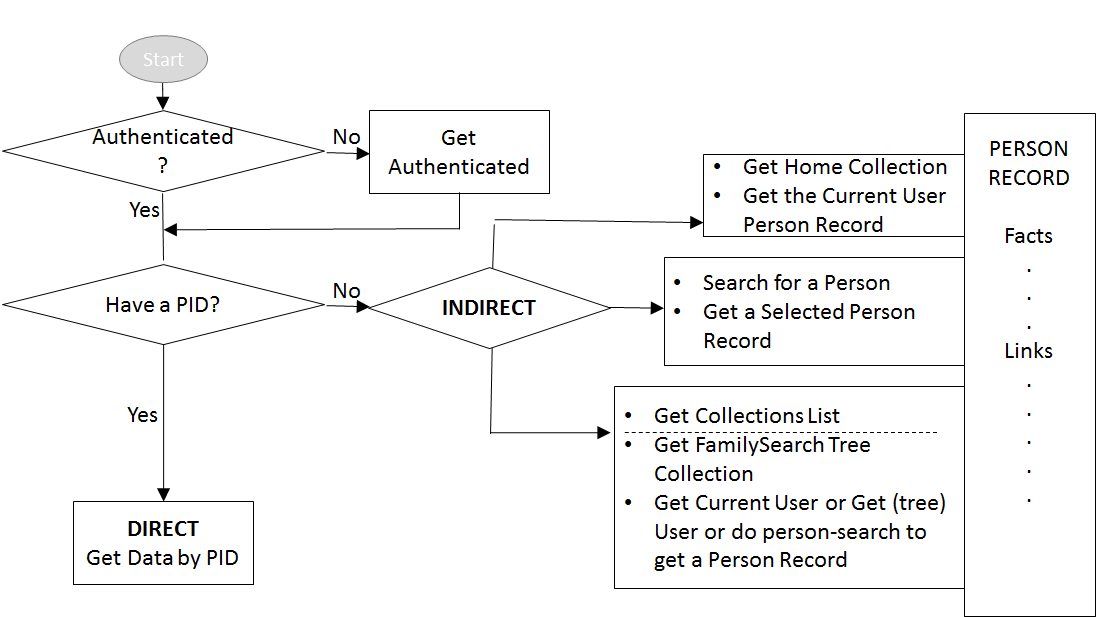
\includegraphics[width=\linewidth]{05/08_dataAccessPaths}
        \centering
        \caption{Sistemes d'accés a les dades de l'arbre familiar}\label{fig:dataAcessPath}
    \end{figure}


    \subsection{L'accés directe a les dades}

        \paragraph{}
        L'accés directe a les dades es pot realitzar si es coneix l'identificador del recurs que vol ser consultat.

        Per exemple, si es coneix el PID de la persona a consultar, es pot codificar des de les aplicacions el diferent conjunt d'URIs per manipular els recursos i evitar així la necessitat de passar pel sistema. D'aquesta forma, es pot doncs accedir a la informació de la persona, memòries, discussions, fills, pares, parelles, avantpassats i descendència; sempre i quan, es conegui tota la informació necessària per codificar les diferents URIs d'accés.

        Un exemple d'ús, podria ser per exemple, donat un identificador de persona conegut, accedir directament a les seves memòries mitjançant la codificació de la URI i evitar, així, haver de passar per l'arbre familiar.


    \subsection{L'accés indirecte a les dades}

        \paragraph{}
        A pesar que poder accedir directament a les dades, pot semblar un procés ideal, el més normal és que ens trobem en la situació de necessitar realitzar un accés indirecte a les dades. En altres paraules, accedir en primera instància als recursos del sistema i obtenir així els diferents enllaços que ens condueixin cap a les operacions desitjades.

        Per descobrir l’URI del recurs exacte que vol ser consultat, existeixen principalment tres opcions diferents:

        \begin{itemize}
            \item Llegir la col·lecció Arrel, que representa la col·lecció que conté totes les dades de FamilySearch i seguir-la per tal d'obtenir l'usuari identificat. Un cop es disposa de la persona relacionada a l'usuari, es pot accedir a qualsevol altre recurs mitjançant els enllaços hypermedia de la resposta i simular, de forma dinàmica, el mateix que podríem haver realitzat mitjançant l'accés directe.
            \item Llegir la llista de col·leccions disponibles per tal d'accedir a l'arbre familiar o accedir a ell de forma directa. Un cop es disposa de l'arbre familiar es pot llegir l'usuari actual o la persona de l'usuari i d'aquí procedir com es desitgi. Una alternativa és accedir mitjançant els enllaços o plantilles URL, als recursos generals de Memòries, Discussions, Relacions, etcètera i consultar la informació general d'aquests recursos mitjançant els seus identificadors retornats.
            \item La tercera opció, i probablement la més comuna, passa per la realització d'una cerca contra la base de dades de FamilySearch per tal d'obtenir una Persona o Localització. Un cop s'obté el resultat de la cerca, es pot navegar a qualsevol de les peces d'informació relacionades als recursos consultats, mitjançant les URI i enllaços hypermedia de les respostes.
        \end{itemize}

        El procés descrit en el tercer punt de les opcions de cerca indirecta, serà el més comú de cara a accedir a la informació, ja que les altres opcions no permeten gaire filtratge de les dades, a menys que coneguem la col·lecció específica sobre la qual volem realitzar una investigació genealògica o només vulguem consultar la informació de l'arbre familiar, de l'usuari identificat.

        Com hem comentat doncs, són quatre les principals opcions d'entrada que permeten obtenir persones concretes de l'arbre de forma indirecta i començar a navegar, des de la resposta d'aquestes, per les dades genealògiques.

        En els següents apartats,  s'explicarà en més detall com poden ser configurades cada una d'aquestes operacions.


    \subsection{Lectura de l'usuari identificat}

        \paragraph{}
        Aquesta operació pot ser realitzada de forma directe, accedint a la URI:

        \begin{displayquote}
            \emph{/platform/users/current}
        \end{displayquote}

        La crida retorna la informació específica del recurs Usuari descrita en els apartats anteriors d'aquesta memòria. Des d'aquest, es pot accedir a la persona de l'arbre familiar que representa a l'usuari i des d’aquesta, a qualsevol altre peça d'informació genealògica relacionada amb la persona.


    \subsection{Lectura de la persona relacionada a l'usuari identificat}

        Aquesta operació és realitzable a través de la URI:

        \begin{displayquote}
            \emph{/platform/tree/current-person}
        \end{displayquote}

        L'operació en qüestió retorna el recurs Persona de l'usuari identificat, amb tota la informació descrita en els apartats anteriors de la memòria. Des d'aquest, es pot navegar a qualsevol altre recurs o dada genealògica relacionada.

        Aquesta forma d'accés representa un pas menys que l’exposada en l’apartat anterior, si sabem d'entrada que volem accedir a l'arbre familiar. En cas que també volguéssim alguna dada del recurs Usuari, caldria entrar per la funcionalitat descrita en l'apartat anterior.


    \subsection{Cerca de Persones a l'arbre familiar}

        \paragraph{}
        L'operació cerca de persones, a l'arbre familiar, és sense cap dubte la més interessant de totes les funcionalitats que ofereix l'API.

        Aquesta operació es realitza mitjançant una petició a la URI /platform/tree/search, que a més a més, pot ser configurada i personalitzada mitjançant la inclusió de diferents paràmetres.

        Un cop finalitzada la petició, aquesta retorna el conjunt de persones de l'arbre familiar, que compleixen amb les condicions imposades en la cerca. L'usuari, pot començar a navegar per la resposta, accedint a aquelles persones que li resultin de més interès i a tots els altres recursos disponibles relacionats amb aquestes.

        Es pot entendre la funcionalitat de cerca a l'arbre familiar, com una porta a totes les dades emmagatzemades per FamilySearch.

        La cerca pot ser controlada mitjançant tres paràmetres principals, un dels quals, accepta molts paràmetres secundaris. Els paràmetres principals són descrits a la taula~\ref{res:searchPersonMain}.

        \begin{center}
                 \csvreader[
                    separator=comma,
                    before table=\sffamily\small,
                    respect tilde=true,
                    respect leftbrace=true,
                    respect rightbrace=true,
                    longtable={p{2cm-2\tabcolsep}p{12cm-2\tabcolsep}},
                    table head={\caption{Variables principals per la cerca de persones}\label{res:searchPersonMain}\\\toprule%
                        \headentry{m{2cm-2\tabcolsep}}{Variable}
                        & \headentry{m{12cm-2\tabcolsep}}{Descripció}\\\midrule},
                    late after line=\\\midrule,
                    late after last line=\\\bottomrule,
                 ]
                 {./tables/05/10_search/searchPersonMain.csv}
                 {var=\var,desc=\desc}
                 {\var&\desc}
         \end{center}

         El paràmetre \emph{q}, descrit en la taula~\ref{res:searchPersonMain}, accepta com a paràmetres vàlids els camps exposats a la taula~\ref{res:searchPersonSec}. L'etiqueta \{relation\}, dels camps d'aquesta taula,  pot ser reemplaçada per qualsevol dels següents valors: father, mother, spouse (pare, mare, parella).

         \begin{center}
                  \csvreader[
                     separator=comma,
                     before table=\sffamily\small,
                     respect tilde=true,
                     respect leftbrace=true,
                     respect rightbrace=true,
                     longtable={p{4cm-2\tabcolsep}p{10cm-2\tabcolsep}},
                     table head={\caption{Paràmetres acceptats per la variable q}\label{res:searchPersonSec}\\\toprule%
                         \headentry{m{4cm-2\tabcolsep}}{Variable}
                         & \headentry{m{10cm-2\tabcolsep}}{Descripció}\\\midrule},
                     late after line=\\\midrule,
                     late after last line=\\\bottomrule,
                  ]
                  {./tables/05/10_search/searchPersonSec.csv}
                  {param=\param,desc=\desc}
                  {\param&\desc}
          \end{center}


          \subsubsection{Cerca de persones duplicades}

          \paragraph{}
          Una característica interessant de les respostes en la cerca de persones és que per cada persona de la resposta, es pot accedir al conjunt de persones de l'arbre familiar, que amb alta probabilitat, poden representar a la mateixa persona consultada. En altres paraules, persones que podrien tractar-se de possibles duplicats.

          Aquesta funcionalitat de cerca de persones duplicades, també es troba accessible mitjançant una URI pròpia, si es coneix l'identificador personal de la persona sobre la qual es vol buscar els possibles duplicats.


    \subsection{Cerca de localitzacions}

        \paragraph{}
        La cerca de localitzacions és la segona opció de cerca massiva que permet l'API de FamilySearch.

        Aquesta operació cobra especial interès quan es necessita consultar informació extra sobre una localització, més enallà de la informació bàsica relacionada a certs recursos de l'arbre familiar, o es vol obtenir informació sobre totes les localitzacions  que compleixen amb certs criteris. Per exemple, totes les localitzacions dins d'una jurisdicció específica.

        Així doncs, la cerca de localitzacions permet relacionar o interpretar, el nom d'una localització, mitjançant una descripció estandarditzada a la URI:

        \begin{displayquote}
            \emph{/platform/places/search}
        \end{displayquote}

        De la mateixa forma que en la cerca de persones, la cerca de localitzacions pot ser configurada mitjançant tres paràmetres principals, on un d'aquests accepta diversos paràmetres secundaris. Els paràmetres principals són descrits a la taula~\ref{res:searchLocMain}.

        \begin{center}
                 \csvreader[
                    separator=comma,
                    before table=\sffamily\small,
                    respect tilde=true,
                    respect leftbrace=true,
                    respect rightbrace=true,
                    longtable={p{2cm-2\tabcolsep}p{12cm-2\tabcolsep}},
                    table head={\caption{Variables principals per la cerca de localitzacions}\label{res:searchLocMain}\\\toprule%
                        \headentry{m{2cm-2\tabcolsep}}{Variable}
                        & \headentry{m{12cm-2\tabcolsep}}{Descripció}\\\midrule},
                    late after line=\\\midrule,
                    late after last line=\\\bottomrule,
                 ]
                 {./tables/05/10_search/searchLocMain.csv}
                 {var=\var,desc=\desc}
                 {\var&\desc}
         \end{center}

         En aquesta operació, el paràmetre \emph{q}, accepta com a vàlids el conjunt de paràmetres especificats a la taula~\ref{res:searchLocSec}.

         \begin{center}
                  \csvreader[
                     separator=comma,
                     before table=\sffamily\small,
                     respect tilde=true,
                     respect leftbrace=true,
                     respect rightbrace=true,
                     longtable={p{2cm-2\tabcolsep}p{10cm-2\tabcolsep}},
                     table head={\caption{Paràmetres acceptats per la variable q}\label{res:searchLocSec}\\\toprule%
                         \headentry{m{2cm-2\tabcolsep}}{Variable}
                         & \headentry{m{10cm-2\tabcolsep}}{Descripció}\\\midrule},
                     late after line=\\\midrule,
                     late after last line=\\\bottomrule,
                  ]
                  {./tables/05/10_search/searchLocSec.csv}
                  {param=\param,desc=\desc}
                  {\param&\desc}
          \end{center}
